\chapter{Results and conclusion}
\label{Chap:Results}

\section{Limits on decay branching fraction}
%The expected upper limits were set with the $CL_{s}$ modified frequentist formalism~\cite{CLs_ref1,CLs_ref2,CLs_ref3} by using the Higgs Combination tool~\cite{CombineToolTwiki}, and was evaluated by asymptotic methods based on the models of the signal and background. 
%No deviation from the background-only hypothesis is observed.
%After full event selections, two muons and a photon are selected to reconstruct Higgs (\cPZ) boson candidates, whose invariant masses $m_{\mu\mu\gamma}$ are used as the observable in the unbinned likelihood computation in the limit setting procedure. 
The distributions in $m_{\mu\mu\gamma}$ observed in the data are in agreement with the SM expectation of the background-only hypothesis.
The results are used to derive upper limits on the branching fractions, $\mathcal{B}(\cPZ\to\JPsi\ \gamma)$ and $\mathcal{B}(\PH\to\JPsi\ \gamma)$ for the $\cPZ$ and Higgs boson.
%No deviation from the background-only hypothesis is observed.
%Hence, upper exclusion limits on the branching fractions, $\mathcal{B}(\PH\to\JPsi\ \gamma)$ and $\mathcal{B}(\cPZ\to\JPsi\ \gamma)$, are set.  
%The exclusion limits are evaluated using the modified frequentist approach, $\text{CL}_\text{s}$, taking the profile likelihood as a test statistic~\cite{CLs_ref1,CLs_ref2,CLs_ref3}. 

The observed (expected) exclusion upper limit on the cross-section times the branching fraction at 95\% CL for the $\PH\to\JPsi\ \gamma$, where the $\JPsi$ meson is fully transversely polarized, is,
\begin{equation}
	\displaystyle
	\sigma(\Pp\Pp\to\PH)\times\mathcal{B}(\PH\to\JPsi\ \gamma\to\mu\mu\gamma)<2.5\ (1.7^{+0.8}_{-0.5})\fb,
	\end{equation}
where upper and lower bounds for 68\% of interval of expected limits are shown as superscript and subscript. 
With the known values of $\sigma(\Pp\Pp\to\PH)=55.1\pb$ and $\mathcal{B}(\JPsi\to\mu\mu) = 0.059$, the above result can be interpreted in terms of limit on  the branching fraction,
\begin{equation}
	\displaystyle
	\mathcal{B}(\PH\to\JPsi\ \gamma)<7.6\ (5.2^{+2.4}_{-1.4})\ten{-4}.
	\end{equation}
which corresponds to 260 (170) times the SM prediction.  

For the $\cPZ$ boson decay, with the unpolarized $\JPsi$ meson assumption ,the observed (expected) upper limit on the cross-section times the branching fraction is,
\begin{equation}
	\displaystyle
	\sigma(\Pp\Pp\to\cPZ)\times\mathcal{B}(\cPZ\to\JPsi\ \gamma\to\mu\mu\gamma)<4.6\ (5.3^{+2.3}_{-1.6})\fb,
	\end{equation}
With the known value $\sigma(\Pp\Pp\to\cPZ)=5.71\times10^{4}\pb$, the observed (expected) upper limit in branching fraction is 
\begin{equation}
	\displaystyle
	\mathcal{B}(\cPZ\to\JPsi\ \gamma)<1.4\ (1.6^{+0.7}_{-0.5})\ten{-6}.
	\end{equation}
, corresponding to 15 (18) times the SM prediction. 

Extreme polarization scenarios give rise to variations from $-13.6\ (-13.5)\%$, for a fully longitudinally polarized $\JPsi$, to $+8.6\ (+8.2)\%$, for a fully transversely polarized $\JPsi$ meson, in the observed (expected) branching fraction.
The observed (expected) exclusion limits on the cross sections and branching fractions at 95\% confidence level for the $\cPZ$ and Higgs boson decays are summarized in Table~\ref{tab:limits_summary}.   

\begin{table}[!ht]
\small
  \setlength{\tabcolsep}{10pt} % Default value: 6pt
  \renewcommand{\arraystretch}{1.3} % Default value: 1
  \begin{center}
    \begin{tabular}{ ccccc }
    Channel & Polarization & $\sigma\ (\text{fb})$ & $\mathcal{B}(\cPZ\ (\PH)\to\JPsi\ \gamma)$ & $\frac{\mathcal{B}(\cPZ\ (\PH)\to\JPsi\ \gamma)}{\mathcal{B}_{\text{SM}}(\cPZ\ (\PH)\to\JPsi\ \gamma)}$\\
    & scenario & & &\\ 
      \hline
      & Unpolarized & $4.6\ (5.3^{+2.3}_{-1.6})$ & $1.4\ (1.6^{+0.7}_{-0.5})\ten{-6}$ & 15 (18) \\
      $\cPZ\to\JPsi\ \gamma$ & Transverse & $5.0\ (5.9^{+2.5}_{-1.7})$ & $1.5\ (1.7^{+0.7}_{-0.5})\ten{-6}$ & 16 (19) \\
      & Longitudinal & $3.9\ (4.6^{+2.0}_{-1.4})$ & $1.2\ (1.4^{+0.6}_{-0.4})\ten{-6}$ & 13 (15) \\
      \hline
      $\PH\to\JPsi\ \gamma$ & Transverse & $2.5\ (1.7^{+0.8}_{-0.5})$ & $7.6\ (5.2^{+2.4}_{-1.6})\ten{-4}$ & 260 (170) \\
      \hline
    \end{tabular}
    \caption{Upper observed (expected) limits on cross sectiona $\sigma (\Pp\Pp\to\cPZ\ (\PH)\to(\JPsi\to\mu\mu)\gamma)\ (\text{fb})$ and branching fractions of $\cPZ\ (\PH)\to\JPsi\ \gamma$ decays, where the latter are computed assuming SM cross section of the $\cPZ\ (\PH)$ boson. Variations of the branching fractions of the $\cPZ$ decay for complete transverse and longitudinal polarizations for $\JPsi$ are also shown. The upper and lower bounds of the expected 68\% confidence level interval for the expected limits are shown as superscripts and subscripts respectively.   \label{tab:limits_summary}}
  \end{center}
\end{table}

\subsection*{Combination with 8\TeV result}
The results of the $\PH\rightarrow\JPsi\ \gamma$ are combined with the results of a similar search performed by the CMS Collaboration using data recorded with $\Pp\Pp$ collisions at $\sqrt{s}=8\TeV$, corresponding to an integrated luminosity of 19.7$\fbinv$~\cite{Run1Paper_Dalitz}. The combination results in an upper limit corresponding to 220 (160) times the SM prediction. All systematic uncertainties are assumed to be uncorrelated in the combination, apart from the theoretical calculations for the cross section and branching fractions. 

\section{Conclusion}
% The observed(expected) exclusion limit at 95\% confidence level on the $\mathcal{B}(\PH\to (\JPsi)\gamma)$ is $7.64\ (5.21^{+2.39}_{-1.57})\times 10^{-4}$, which corresponds to 255 (174) times the SM value, and on the $\mathcal{B}(\cPZ\to (\JPsi)\gamma)$ is $1.35(1.58^{+0.67}_{-0.47})\times 10^{-6}$, assuming unpolarized $\JPsi$, which corresponds to 15.1 (17.7) times its SM prediction. 
%The results for the Higgs boson decay are combined with the results from pp collisions at $\sqrt{s}=8~\TeV$ corresponding to 19.7~\fbinv and this results in an expected (observed) upper limit on the branching fraction for $\PH\to(\JPsi)\gamma$ of 221(158) times the standard model prediction.
%In the Z decay, extreme polarization scenarios give rise to a variation from -13.6(-13.5)\%, for a fully longitudinally polarized $\JPsi$, to +8.57(+8.21)\%, for a fully transversely polarized $\JPsi$, on the observed(expected) branching ratio. 

%A search is performed for the decays of the SM $\cPZ$ and Higgs bosons into a $\JPsi$ and a photon with $\JPsi$ subsequently decaying into $\PGmp\PGmm$. No excess has been observed above the predicted background. 
%The limit on the branching ratio of the Higgs boson is set at $\mathcal{B}(\PH\to\JPsi\ \gamma)<7.64\ (5.21^{+2.39}_{-1.57})\times 10^{-4}$, corresponding to 255 (174) times the SM value. The upper and lower bounds for 68\% of interval of expected limits are shown as superscript and subscript. 
%The results for the Higgs boson decay are combined with the results from $\Pp\Pp$ collisions at $\sqrt{s}=8\TeV$ corresponding to 19.7\fbinv and this results in an expected (observed) upper limit on the branching fraction for $\PH\to\JPsi\ \gamma$ of 221(158) times the SM prediction. It is worth noting that the current sensitivity of the $\PH\to\JPsi\ \gamma$ search is compatible to the $\PH\to\ccbar$ search from the ATLAS Collaboration. 
%The observed (expected) exclusion limit at 95\% confidence level on the branching ratio of the $\cPZ$ boson decay in the unpolarized scenario is set at $\mathcal{B}(\cPZ\to\JPsi\ \gamma) < 1.35\ (1.58^{+0.67}_{-0.47})\times 10^{-6}$, corresponding to 15.1 (17.6) times its SM prediction. 
%Extreme polarization scenarios give rise to variations from -13.6 (-13.5)\%, for a fully longitudinally polarized $\JPsi$, to +8.6 (+8.2)\%, for a fully transversely polarized $\JPsi$, on the observed (expected) branching fraction. 
A search is performed for decays of the standard model (SM) $\cPZ$ and Higgs bosons into a $\JPsi$ meson and a photon with the $\JPsi$ meson subsequently decaying into $\PGm\PGm$. 
Data from $\Pp\Pp$ collisions at $\sqrt{s}=13\TeV$, corresponding to an integrated luminosity of 35.9\fbinv is used.
No excess has been observed above the predicted background. 
The observed (expected) exclusion limit at 95\% CL on the branching fraction of the Higgs boson is set at $\mathcal{B}(\PH\to\JPsi\ \gamma)<7.6\ (5.2)\ten{-4}$, corresponding to 260 (170) times the SM value. The 68\% confidence level interval ranges from 3.6 to 7.6$\times 10^{-4}$.
The limit on the branching fraction of the $\cPZ$ boson decay in the unpolarized scenario is set at $\mathcal{B}(\cPZ\to\JPsi\ \gamma) < 1.4\ (1.6)$, corresponding to 15 (18) times the SM prediction. The 68\% confidence level interval ranges from 1.1 to 2.3$\times 10^{-6}$.
Extreme polarization scenarios give rise to variations from $-13.6\ (-13.5)\%$, for a fully longitudinally polarized $\JPsi$ meson, to $+8.6\ (+8.2)\%$, for a fully transversely polarized $\JPsi$ meson, in the observed (expected) branching fraction. 
The results for the Higgs boson channel are combined with the results obtained by a similar search performed at $\sqrt{s}=8\TeV$ by the CMS Collaboration, yielding an observed (expected) upper limit on the branching fraction for the decay $\PH\to\JPsi\ \gamma$ of 220 (160) times the SM prediction.

\section{Outlook}
Improvements can be done in order to make the analysis more advanced. The proper simulation of the background processes is of the first priority. The difficulty is mainly due to the large cross sections of the low mass dimuon system in the final states, and therefore efficient ways to produce such samples should be developed. The background samples will enable us to have better understanding of the background composition and make the optimization of the event selection feasible. Furthermore, the multivariate analysis (MVA) or the matrix element method\footnotemark (MEM) can be exploited to better discriminate the signal and background. 
\footnotetext{For example, the Matrix Element Likelihood Analysis (MELA) used in the $\PH\to\cPZ\cPZ^{*}\to 4l$ analysis. }
The analysis can be extended to include the decay of $\cPZ(\PH)\to\Upsilon(\text{nS})\gamma$, where the $\Upsilon(\text{nS})$ mesons decay to a muon pair.  The one dimension fit in the $m_{\mu\mu\gamma}$ space to estimate the background in this analysis will need to be modified to cope with the non-negligible contribution of the peaking background $\cPZ\to\mu\mu\gamma$. A two dimension (in the $m_{\mu\mu}$ and $m_{\mu\mu\gamma}$ space) or multi-dimension fit is suggested. The background composition can also be estimated by this data-driven method, and in turn can be used to validate the background simulation samples. The development of the identification and reconstruction of merged electrons can be used in the electron channel. The projection study is performed, and the expected distributions of $m_{\mu\mu\gamma}$ with $3000\fbinv$ of data from both decay channels are shown in Fig.~\ref{fig:projection}. The upper limit on $\mathcal{BR}(\cPZ\to\JPsi\ \gamma)$ is around 2 times its SM value, while that on the $\mathcal{BR}(\PH\to\JPsi\ \gamma)$ is expected to be less than 20 times its SM prediction. With the addition of the electron channel and foreseeable improvements, the $\cPZ\to\JPsi\ \gamma$ would be sensitive to it's current SM predicted rate after the high luminosity run of the LHC, possibly leading to the first observation of this rare decay of the $\cPZ$ boson.

\begin{figure}[!ht]
\begin{center}
	  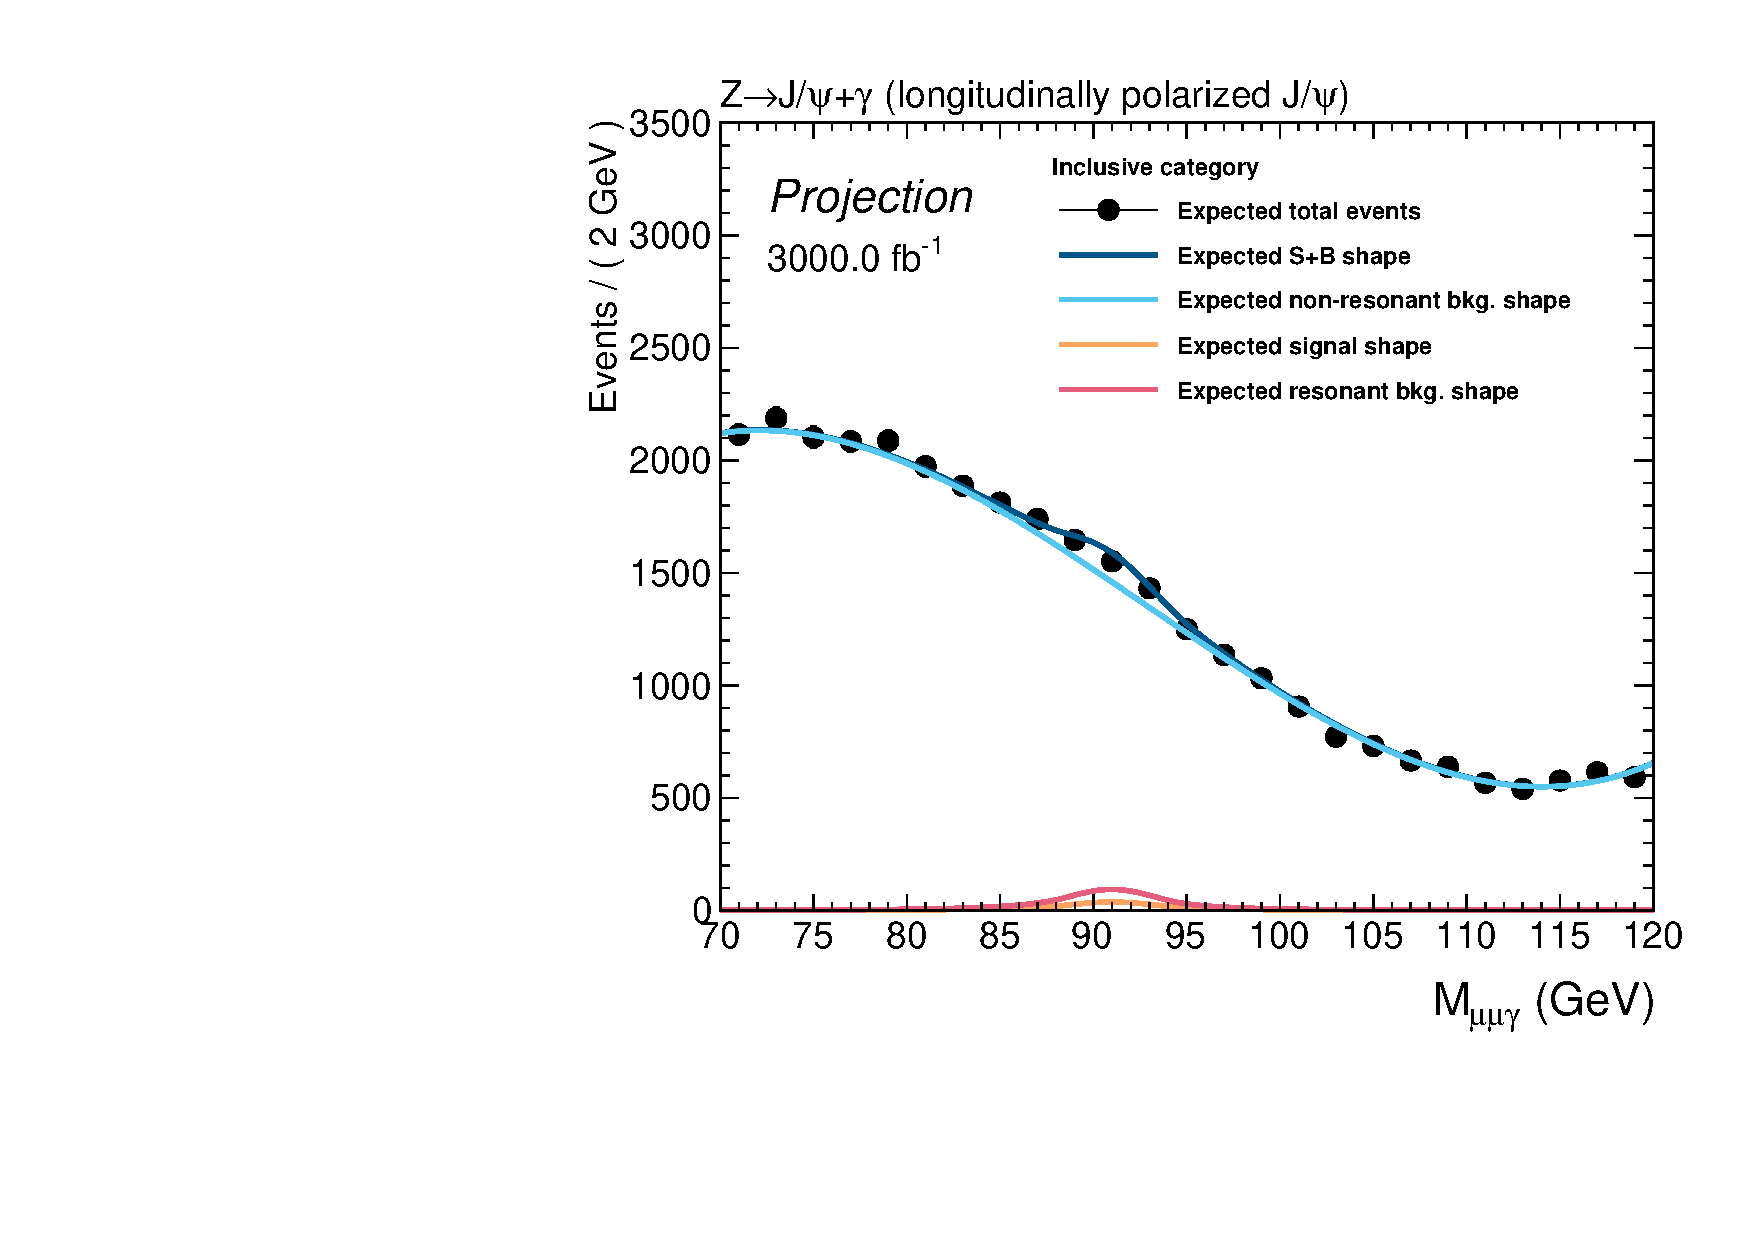
\includegraphics[width=0.5\textwidth]{Fig/projection/ZJpsiG_data_Inclusive_cat1_longipolarized_proj_3000invfb}~
	  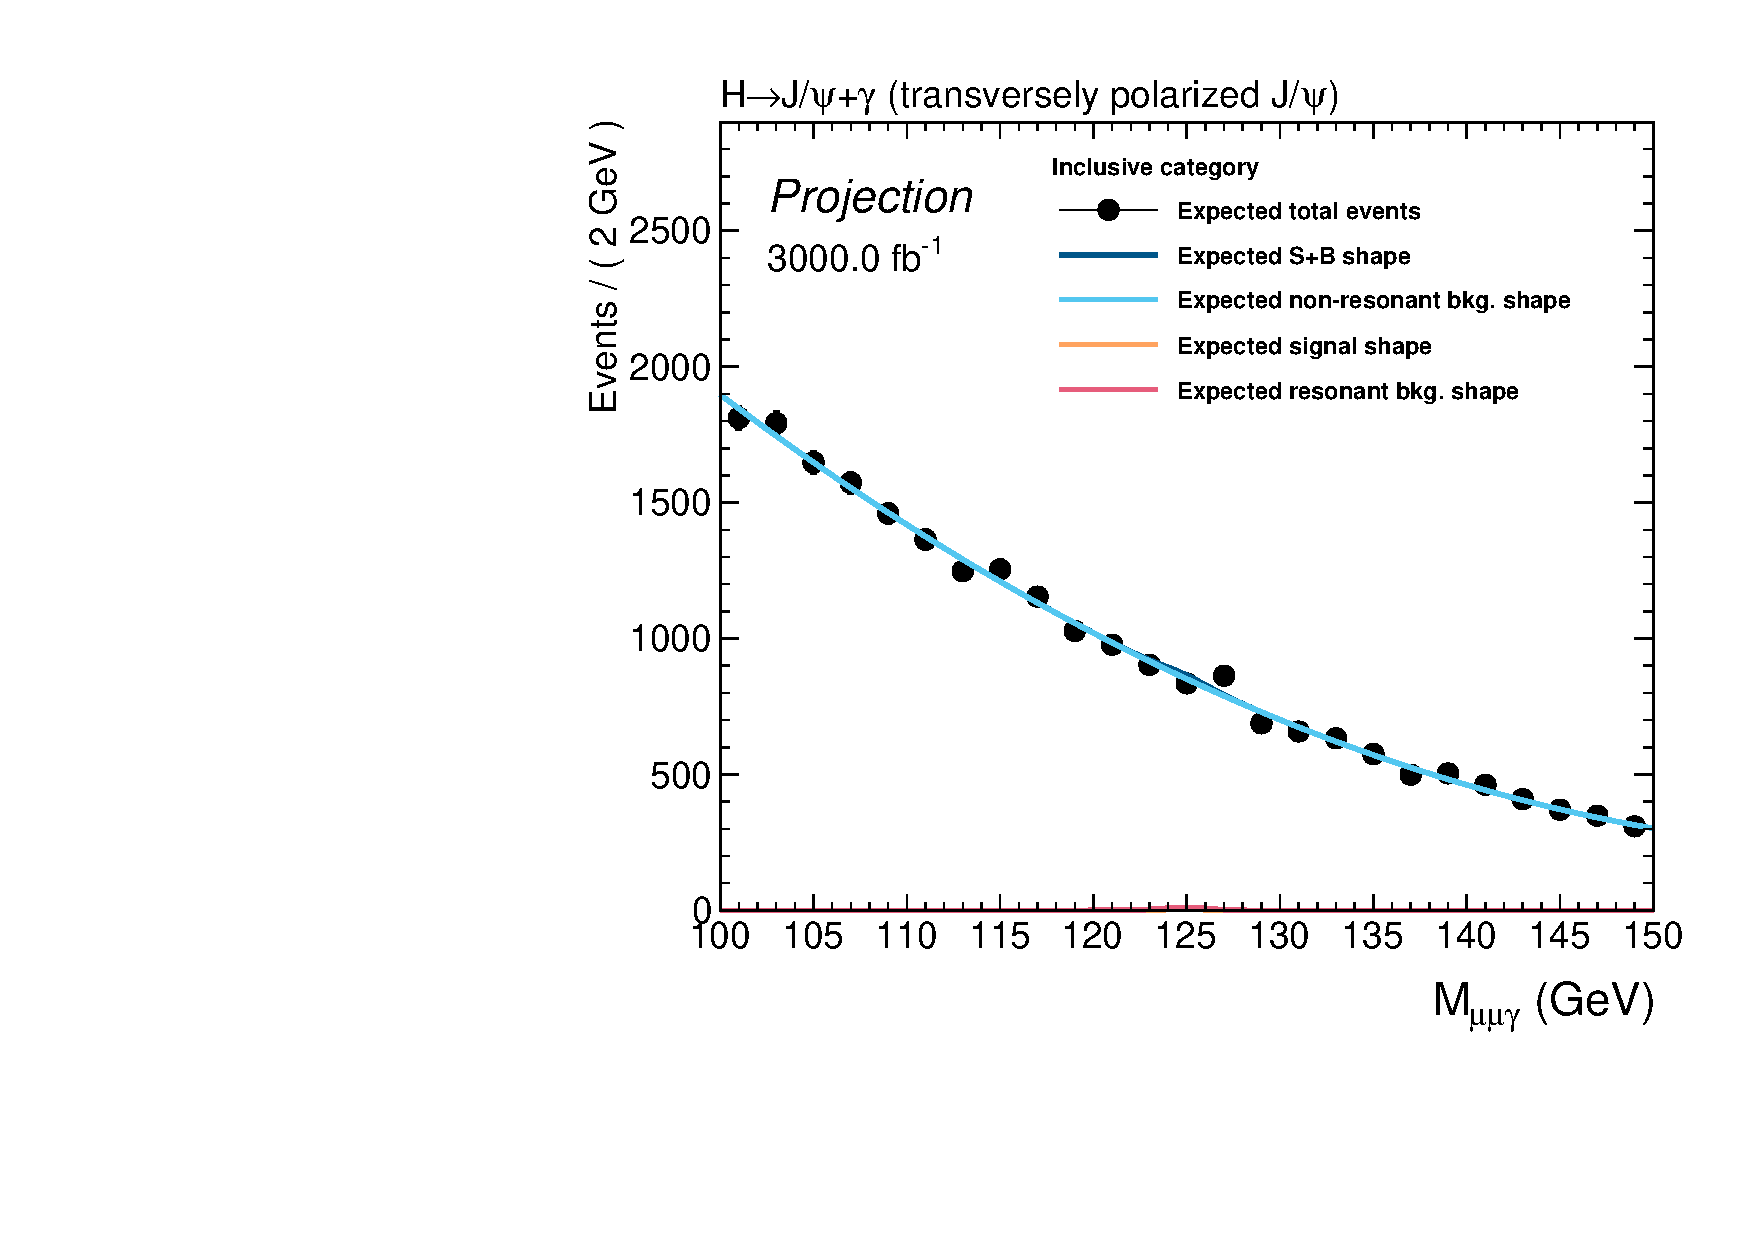
\includegraphics[width=0.5\textwidth]{Fig/projection/HJpsiG_data_Inclusive_cat1_transpolarized_proj_3000invfb}\\
	  \caption{The expected distributions of $m_{\mu\mu\gamma}$ at $3000\fbinv$ of data from both decay channels.\label{fig:projection}}
\end{center}
\end{figure}
